\documentclass{beamer}
\usetheme{Boadilla}

\usepackage{graphicx}
\usepackage{tikz}

\usetikzlibrary{positioning, arrows.meta, calc, fit, shapes, decorations.pathreplacing, backgrounds}
\tikzstyle{fancytitle} =[fill=white, text=black, draw]

\definecolor{colorThree}{HTML}{CC6633}
\definecolor{tikzDarkGreen}{HTML}{006622}
\definecolor{tikzBack}{HTML}{e0e0eb}

\setbeamertemplate{note page}[plain]
%\setbeameroption{show notes}

\title[Reconstructing MetiTarski Proofs in Isabelle]{Reconstructing MetiTarski Proofs in Isabelle/HOL}
\subtitle {End-of-internship Presentation}
\author{Cristina Matache}
\institute[]{
\includegraphics[scale=0.45]{ai_logo_title}}
\date{September 22, 2017}

%Remove the navigation buttons
\setbeamertemplate{navigation symbols}{}

\begin{document}

\begin{frame}
\titlepage
\end{frame}

\begin{frame}
\frametitle{Outline}
\tableofcontents
\end{frame}

\section{MetiTarski}

\begin{frame}
\frametitle{MetiTarski}
\begin{itemize}
\item Automatic theorem prover (ATP)
\item Proves universally quantified inequalites involving:
	\begin{itemize}
	\item polynomials
	\item real-valued special functions: $log$, $exp$, $sin$, $cos$, $sqrt$ etc.
	\end{itemize}
\item Using:
	\begin{itemize}
	\item resolution
	\item a decision procedure for the theory of real closed fields (RCF)
	\end{itemize}
\item The special functions are \textit{approximated} by polynomials. So Metitarski is incomplete. (Without the approximations, the problem is undecidable.)			
\end{itemize}
\end{frame}

\begin{frame}
\frametitle{Motivation}

\begin{itemize}
\item Long-term goal: use MetiTarski inside Imandra to solve geometric problems
	\note[item]{These can be encoded as inequalities that MT understands.}
	
\item Why translate MetiTarski proofs to Isabelle proofs?
	\note[item]{If we want to use MT to verify things, we need very high confidence in its proofs.}
\begin{itemize}
\item No formal guarantee that the MetiTarski proofs are correct.
	\note[item]{MetiTarski was coded in Standard ML and there is no guarantee the code or the output is correct. Although it has of course been tested.}
\item Isabelle is more trustworthy than MetiTarski
\item If proof reconstruction is available, MetiTarski can be included as an automated tool in Isabelle
\end{itemize}
\end{itemize}
\end{frame}

\begin{frame}
\frametitle{The Problem}

\begin{minipage}{0.3\linewidth}
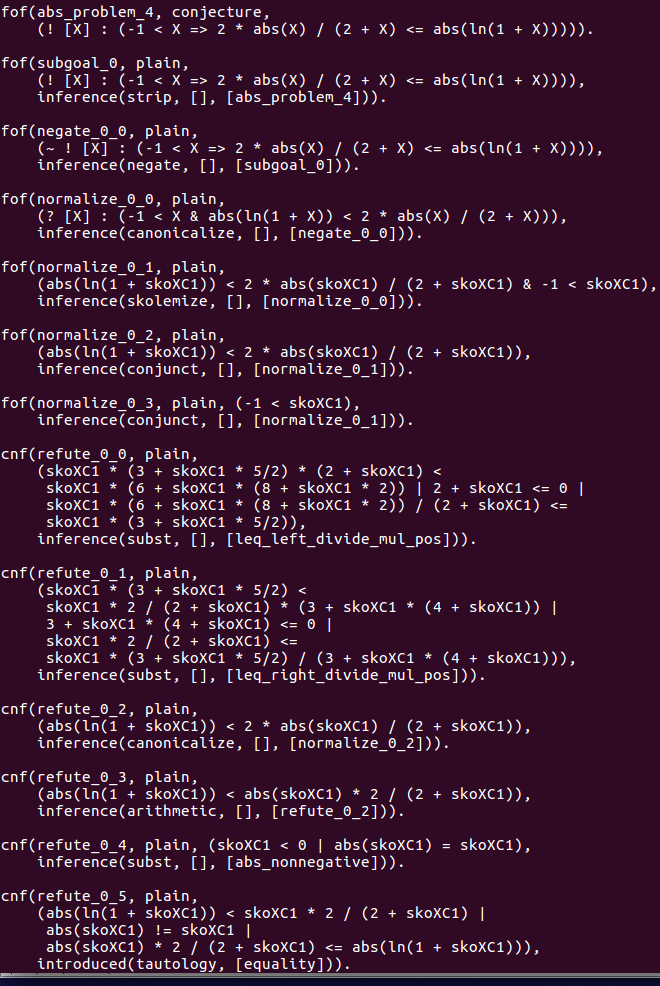
\includegraphics[scale=0.2]{MT_proof}
\end{minipage}
\hfill
\begin{minipage}{0.57\linewidth}
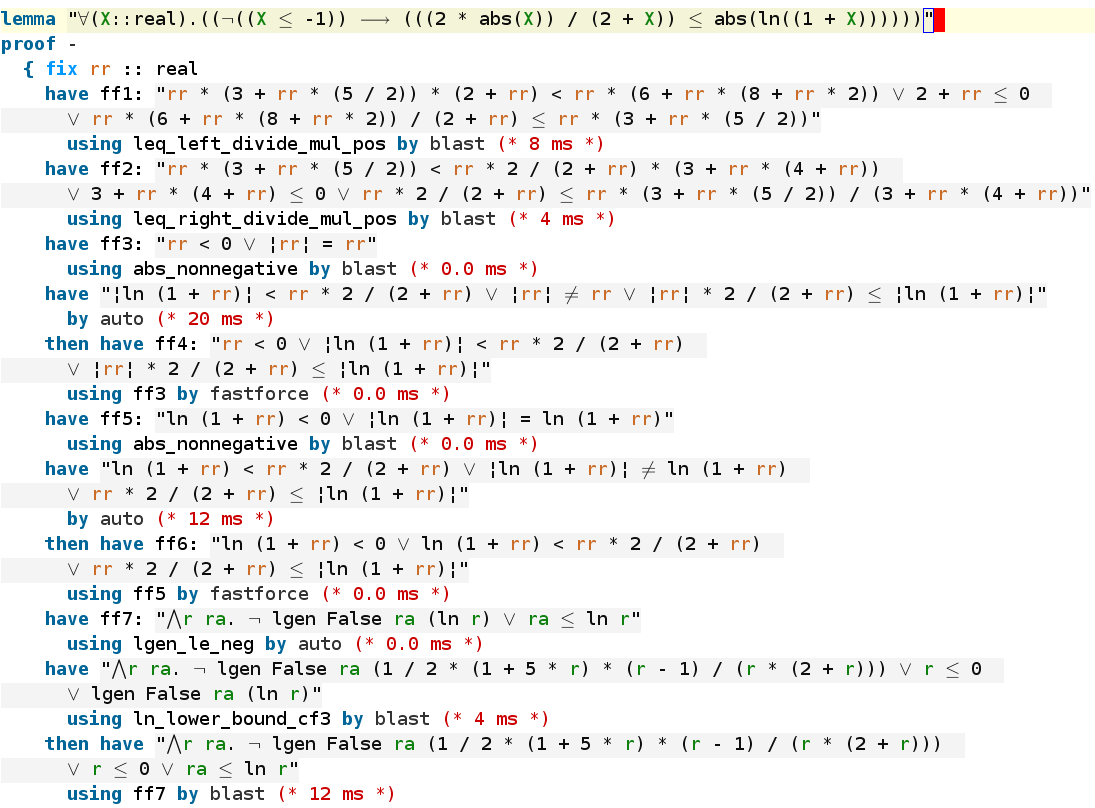
\includegraphics[scale=0.18]{isabelle_proof}
\end{minipage}

%Side by side picture of an MT and Isabelle proofs
	\note[item]{We need to turn this MT proof into an Isabelle proof. You don't need to read all of this, the point is that MT ouputs the steps in a proof, and we want to translate each step to to a "have" in Isabelle. In Isabelle you can specify intermediate proof steps using "have". Each accompanied by a proof method.}
\end{frame}

\section{Sledgehammer}

\begin{frame}
\frametitle{Sledgehammer}

\begin{itemize}
\setlength\itemsep{1em}
\item Automatic proof tool in Isabelle.
	\note[item] {It turns out there is a tool in Isabelle that does something similar. Isabelle is an \textit{interactive} theorem prover so it normally requires a lot of user input to do a proof, the user has to specify what steps should be taken. Sledgehammer aims to improve automation.}
	
	\note[item] {Sledgehammer tries to automatically find a proof for the given lemma without any user input. What it does is it calls a bunch of ATPs and tries to translate their proofs into Isabelle proofs. Which is exactly what I need to do.}

\item Sledgehammer operation:
\end{itemize}

	
\begin{figure}	
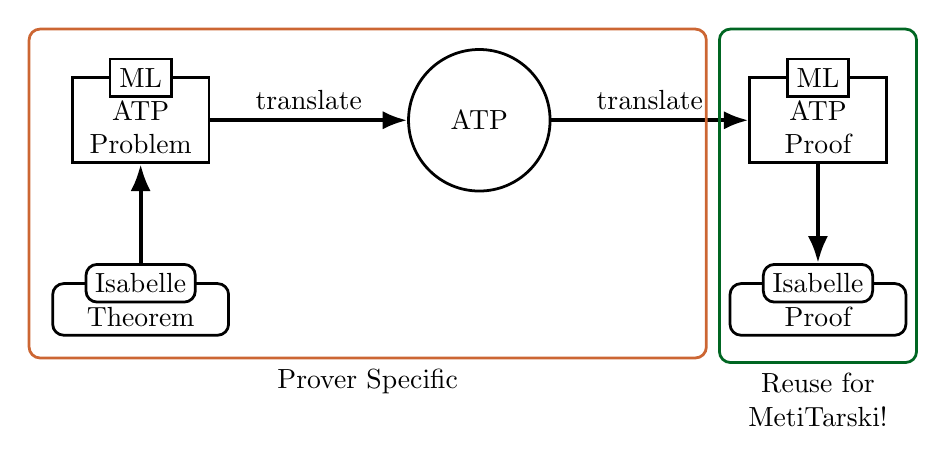
\begin{tikzpicture}
\node (atpProb) [align = center, text width = 1.5cm, draw, line width=1pt] {\\ATP Problem};
\node (atpProbTitle) [fancytitle, above=-0.27cm, line width=1pt] at (atpProb.north) {ML};

\node (isa) [align = center, text width = 2cm, draw, rounded corners, line width=1pt, below=1.5cm of atpProb] {\\Theorem};
\node (isaTitle) [fancytitle, rounded corners, above=-0.27cm, line width=1pt] at (isa.north) {Isabelle};

\node (atp) [circle, align = center, text width = 1.5cm, draw, line width=1pt, right=2.5cm of atpProb] {ATP};

\node (atpProof) [align = center, text width = 1.5cm, draw, line width=1pt, right=2.5cm of atp] {\\ATP Proof};
\node (atpProofTitle) [fancytitle, above=-0.27cm, line width=1pt] at (atpProof.north) {ML};

\node (isaProof) [align = center, text width = 2cm, draw, rounded corners, line width=1pt, below=1.5cm of atpProof] {\\Proof};
\node (isaProofTitle) [fancytitle, rounded corners, above=-0.27cm, line width=1pt] at (isaProof.north) {Isabelle};

\draw[-{Latex},line width=1.5pt, black]
	(isaTitle) edge (atpProb);

\draw[-{Latex},line width=1.3pt, black]
	(atpProb) edge
		node [align = center, text width = 1.5cm, above] {translate} 
	(atp);
	
\draw[-{Latex},line width=1.3pt, black]
	(atp) edge
		node (trans) [align = center, text width = 1.5cm, above] {translate} 
	(atpProof);	

\draw[-{Latex},line width=1.5pt, black]
	(atpProof) edge (isaProofTitle);

\node (box1) [fit={($(isa)+(-1.3cm, -0.5cm)$) ($(trans)-(-0.6cm, 0cm)$) ($(atpProbTitle)+(0cm, 0.5cm)$)}, draw, rounded corners, color=colorThree, line width = 1pt] {};

\node [align = center, text width = 3cm, below=0cm of box1] {Prover Specific};

\node (box2) [fit={(isaProof) ($(isaProofTitle)+(0cm, -0.89cm)$) ($(atpProofTitle)+(0cm, 0.5cm)$)}, draw, rounded corners, color=tikzDarkGreen, line width = 1pt] {};

\node [align = center, text width = 2cm, below=0cm of box2] {Reuse for MetiTarski!};

\end{tikzpicture}
\end{figure}

	\note[item] {When the user invokes Sledgehammer the current goal is translated into some intermediate form, this ATP problem, which is an ML datastructure. This is given to the ATP, it comes up with a proof, which you can put into this standard format of an ATP proof, and then translate it to an Isabelle proof. This is of course a simplified diagram of what happens but you get the idea.}
	\note[item] {The left part of the diagram is specific to every prover, because to get the ATP proof we need some information about how the initial Isabelle lemma was encoded. And this of course depends on each prover. But the right part of the diagram does not depend on the prover. And it is actually the more involved part. So the idea was to somehow reuse this part when reconstructing Metitarski proofs.}

\end{frame}

\begin{frame}
\frametitle{The Translation}
	\note[item] {I'm going to focus first on the left side of the diagram before. The part I said was prover specific.}
	\note[item] {Because Isabelle is written in SML, any code that wants to access the Isabelle internals, for example the internal representation of lemmas, needs to go through SML. So all of the code for this diagram is in SML.}

\begin{figure}
\scalebox{0.4}{
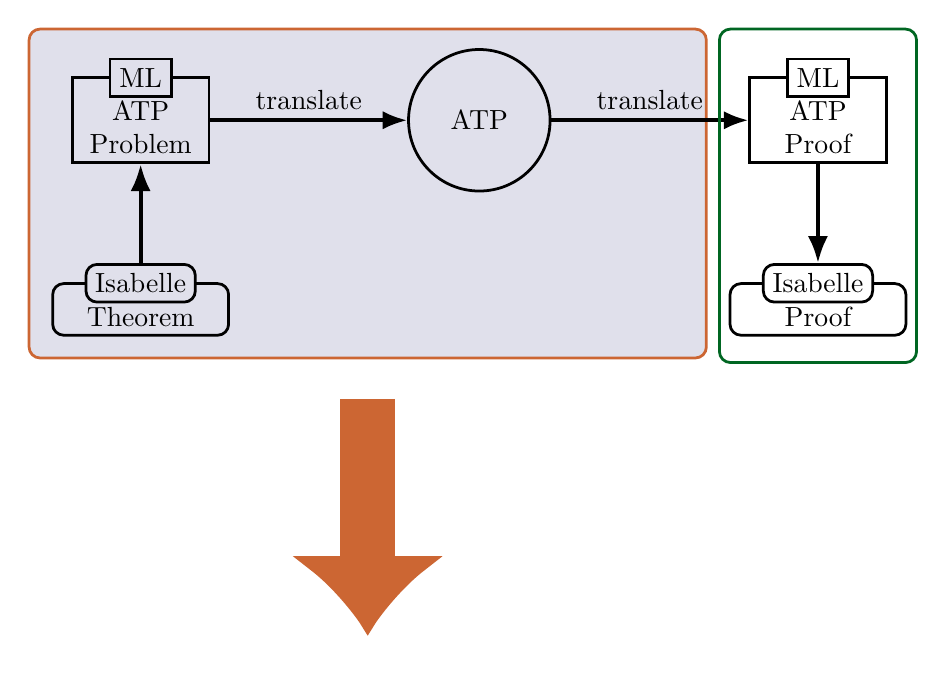
\begin{tikzpicture}
\node (atpProb) [align = center, text width = 1.5cm, draw, line width=1pt] {\textcolor{black}{\\ATP Problem}};
\node (atpProbTitle) [fancytitle, above=-0.27cm, line width=1pt, fill=tikzBack] at (atpProb.north) {ML};

\node (isa) [align = center, text width = 2cm, draw, rounded corners, line width=1pt, below=1.5cm of atpProb] {\\Theorem};
\node (isaTitle) [fancytitle, rounded corners, above=-0.27cm, line width=1pt, fill=tikzBack] at (isa.north) {Isabelle};

\node (atp) [circle, align = center, text width = 1.5cm, draw, line width=1pt, right=2.5cm of atpProb] {ATP};

\node (atpProof) [align = center, text width = 1.5cm, draw, line width=1pt, right=2.5cm of atp] {\\ATP Proof};
\node (atpProofTitle) [fancytitle, above=-0.27cm, line width=1pt] at (atpProof.north) {ML};

\node (isaProof) [align = center, text width = 2cm, draw, rounded corners, line width=1pt, below=1.5cm of atpProof] {\\Proof};
\node (isaProofTitle) [fancytitle, rounded corners, above=-0.27cm, line width=1pt] at (isaProof.north) {Isabelle};

\draw[-{Latex},line width=1.5pt, black]
	(isaTitle) edge (atpProb);

\draw[-{Latex},line width=1.3pt, black]
	(atpProb) edge
		node [align = center, text width = 1.5cm, above] {translate} 
	(atp);
	
\draw[-{Latex},line width=1.3pt, black]
	(atp) edge
		node (trans) [align = center, text width = 1.5cm, above] {translate} 
	(atpProof);	

\draw[-{Latex},line width=1.5pt, black]
	(atpProof) edge (isaProofTitle);

\begin{scope}[on background layer]
\node (box1) [fit={($(isa)+(-1.3cm, -0.5cm)$) ($(trans)-(-0.6cm, 0cm)$) ($(atpProbTitle)+(0cm, 0.5cm)$)}, draw, rounded corners, color=colorThree, line width = 1pt, fill=tikzBack] {};
\end{scope}

%\node [align = center, text width = 3cm, below=0cm of box1] {Prover Specific};

\node (box2) [fit={(isaProof) ($(isaProofTitle)+(0cm, -0.89cm)$) ($(atpProofTitle)+(0cm, 0.5cm)$)}, draw, rounded corners, color=tikzDarkGreen, line width = 1pt] {};

%\node [align = center, text width = 2cm, below=0cm of box2] {Reuse for MetiTarski!};

%arrow
\draw[-{Latex[width=2cm, length=1cm]},line width=20pt, colorThree]
	($(box1.south)+(0, -0.5cm)$) -- ++(0, -3cm);

\end{tikzpicture}
}

\scalebox{0.7}{
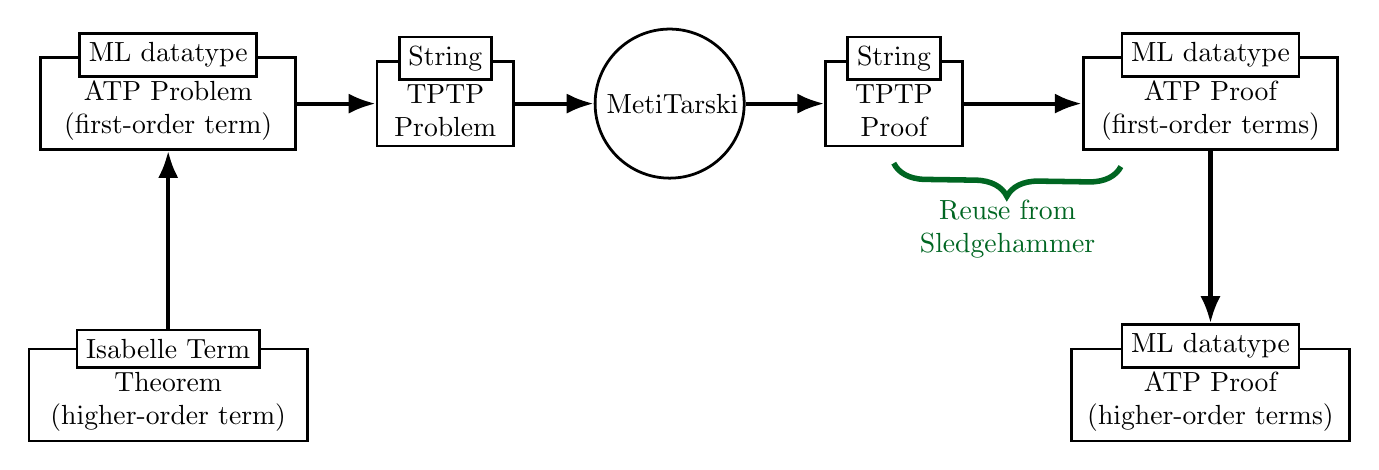
\begin{tikzpicture}
\node (atpProb) [align = center, text width = 3cm, draw, line width=1pt] {\\ATP Problem (first-order term)};
\node (atpProbTitle) [fancytitle, above=-0.27cm, line width=1pt] at (atpProb.north) {ML datatype};

\node (isa) [align = center, text width = 3.3cm, draw, line width=1pt, below=2.5cm of atpProb] {\\Theorem\\ (higher-order term)};
\node (isaTitle) [fancytitle, above=-0.27cm, line width=1pt] at (isa.north) {Isabelle Term};

\node (tptpProb) [align = center, text width = 1.5cm, draw, line width=1pt, right= of atpProb] {\\TPTP Problem};
\node (tptpProbTitle) [fancytitle, above=-0.27cm, line width=1pt] at (tptpProb.north) {String};

\node (atp) [circle, align = center, text width = 1.6cm, draw, line width=1pt, right=1cm of tptpProb] {MetiTarski};

\node (tptpProof) [align = center, text width = 1.5cm, draw, line width=1pt, right=1cm of atp] {\\TPTP Proof};
\node (tptpProofTitle) [fancytitle, above=-0.27cm, line width=1pt] at (tptpProof.north) {String};

\node (atpProof) [align = center, text width = 3cm, draw, line width=1pt, right=1.5cm of tptpProof] {\\ATP Proof (first-order terms)};
\node (atpProofTitle) [fancytitle, above=-0.27cm, line width=1pt] at (atpProof.north) {ML datatype};

\node (atpProofTerm) [align = center, text width = 3.3cm, draw, line width=1pt, below=2.5cm of atpProof] {\\ATP Proof\\ (higher-order terms)};
\node (atpProofTermTitle) [fancytitle, above=-0.27cm, line width=1pt] at (atpProofTerm.north) {ML datatype};

\draw[-{Latex},line width=1.5pt, black]
	(isaTitle) edge (atpProb);
	
\draw[-{Latex},line width=1.5pt, black]
	(atpProb) edge (tptpProb);
	
\draw[-{Latex},line width=1.5pt, black]
	(tptpProb) edge (atp);
	
\draw[-{Latex},line width=1.5pt, black]
	(atp) edge (tptpProof);
	
\draw[-{Latex},line width=1.5pt, black]
	(tptpProof) edge (atpProof);
	
\draw[-{Latex},line width=1.5pt, black]
	(atpProof) edge (atpProofTermTitle);
	
%brace
\draw[decoration={brace,raise=0.2cm, amplitude=0.4cm, mirror},decorate, line width = 2pt, color=tikzDarkGreen]
	  (tptpProof.south) -- 
	  	node[align = center, below=0.5cm, text width=2.5cm] {Reuse from Sledgehammer} 
	  ($(atpProof.south west)+(0.5cm, 0cm)$);						
\end{tikzpicture}
}	
\end{figure}	
	
\end{frame}

\begin{frame}
\frametitle{Generating Isabelle Proofs}
	\note[item] {This is the part we decided to reuse, the right of the diagram. This already has a lot of sophisticated functionality implemented, apart from the textual translation. Explain each of it.}
	\note[item] {It takes the termified ATP proof and translates it to this:}
	\note[item] {But what is difficult is choosing the appropriate proof method for each step in the proof. Because this depends on what steps the prover made. So I had to change the Sledgehammer code to for the MT proofs to work.}
\end{frame}

\begin{frame}
\frametitle{MetiTarski Proof Steps}
\begin{enumerate}
\item \texttt{decision}: invokes the RCF decision procedure
\item \texttt{arithmetic}: algebraic simplification
\end{enumerate}
\end{frame}

\begin{frame}
\frametitle{Summary}
\begin{itemize}
\item What's been done:
	\begin{itemize}
	\item Translation from Isabelle Lemmas to termified ATP Proofs
	\item 
	\end{itemize}
\item Still to do:
	\begin{itemize}
	\item 
	\end{itemize}		
\end{itemize}
\end{frame}

\end{document}